\pdfoutput=1
\documentclass[conference]{IEEEtran}

\usepackage[utf8]{inputenc}
\usepackage[T1]{fontenc}
\usepackage{amsmath,amssymb,amsfonts}
\usepackage{graphicx}
\usepackage{booktabs}
\usepackage{multirow}
\usepackage{hyperref}
\usepackage{xcolor}
\usepackage{microtype}

\graphicspath{{figures/}}

\title{PPC-Gauge-Triad v0.7: Deterministic \texttt{\#![no\_std]} Streaming Anomaly Detection with $Sim^+(d)$ Givens-QR Canonicalization and On-Chip Zero-Touch Auto-Warmup under 16\,KB SRAM}

\author{
  \IEEEauthorblockN{Imlevion}
  \IEEEauthorblockA{PPC-Gauge-Triad Project\\
  Repository: \url{https://github.com/Imlevion/ppc-gauge-triad}}
}

\begin{document}

\maketitle

\begin{abstract}
Real-time anomaly detection on resource-constrained microcontrollers and compact edge telemetry gateways requires deterministic execution, strictly bounded static SRAM, zero dynamic heap allocation, and robustness to physical nuisance transformations such as sensor re-orientation, gain scaling, and thermal baseline drift. We present \textbf{PPC-Gauge-Triad v0.7} (\texttt{ppc\_gauge\_triad\_rs}), a deterministic \texttt{\#![no\_std]} single-precision (\texttt{f32}) Rust streaming engine operating on multi-channel windows $X_t \in \mathbb{R}^{w \times d}$ ($w=8, d=4$) with \textbf{0\,B heap allocation} and \textbf{0 matrix inversions}. The engine decomposes each window into three orthogonal gauge channels: (i) canonical shape $s_{\text{shape}}$ via orthonormal temporal DCT-II projection, explicit $2\times 2$ Givens-QR canonicalization on the proper similarity group $Sim^+(d)$ ($\det=+1$, preserving chirality sensitivity under reflections), and a symmetrized $K$-prototype rank-1 Sherman--Morrison precision bank ($K \le 4$); (ii) log-fluctuation energy $s_{\text{energy}}$; and (iii) per-channel DC level $s_{\text{level}}$ with dual-mode Huber-clamped EMA (server telemetry) or stable-plateau re-lock (embedded thermal sensors) coupled with a dual-stage alarm gate. In v0.7, we introduce \texttt{AutoCalBufF32}, a fixed-size \texttt{\#![no\_std]} on-chip state machine (\texttt{Warmup} $\to$ \texttt{Calibrate} $\to$ \texttt{Monitor}) that computes split-conformal quantiles and $\log(1+\cdot)$-MAD normalizers directly inside static memory, yielding a combined static struct footprint of \textbf{14,744\,B (14.40\,KB)} on ARM Cortex-M4F (\texttt{thumbv7em-none-eabihf}) and \textbf{14,768\,B (14.42\,KB)} on 64-bit hosts (enforced $<16$\,KB at compile time). Across 9/9 pre-registered Level~1 algorithmic tests, 8 real-world SMD/PSM servers, OpenML physical trajectory benchmarks, and 50,000-window 5-seed streaming audits, locked \emph{a priori} presets achieve \textbf{78.7\%} mean AUROC (High-Recall), \textbf{7.6\%} mean FAR (Low-FAR), \textbf{0.30\% $\pm$ 0.13\%} FAR with \textbf{100.0\%} fault recall under multi-regime streaming, and \textbf{75.3\%--82.9\%} mean AUROC via zero-touch on-chip auto-warmup (100--400 normal windows, 0 labels). We explicitly document per-device unsupervised warmup as a design requirement (pure zero-shot cross-device transfer scores 29.7\%) and position physical MCU silicon verification (Level~3) as pending external hardware measurement via an open Cortex-M4F DWT evaluation template.
\end{abstract}

\begin{IEEEkeywords}
streaming anomaly detection, embedded Rust, no\_std, similarity invariance, Givens QR, Sherman--Morrison, split conformal prediction, edge telemetry
\end{IEEEkeywords}

\section{Introduction}
Streaming anomaly detectors deployed on industrial microcontrollers, physical sensor nodes, and low-overhead telemetry agents face a stringent intersection of mathematical and systems constraints. Physically, multi-channel sensor streams undergo nuisance transformations---mounting rotations $Q \in SO(d)$, calibration gain changes $s > 0$, and thermal or workload DC offsets---while chiral inversions ($\det Q = -1$, e.g., axis sign flips or wiring reversals) often represent genuine physical faults that Gram-matrix methods cannot detect. Operationally, embedded firmware frequently prohibits heap allocation (\texttt{\#![no\_std]}), floating-point matrix inversions, and cloud round-trips, demanding predictable $<16$\,KB static SRAM budgets.

Deep sequence models and offline kernel baselines assume unconstrained cloud memory and batch retraining, while lightweight univariate heuristics discard cross-channel geometric structure. \textbf{PPC-Gauge-Triad} bridges this gap through an orthogonal 3-channel gauge decomposition combined with rank-1 online precision updates~\cite{sherman1950} and finite-sample split-conformal calibration~\cite{vovk2005conformal}.

Our evidence-aligned contributions in v0.7 are:
\begin{enumerate}
  \item \textbf{Exact $Sim^+(d)$ Canonicalization with Chirality Preservation:} Temporal DCT-II projection and explicit $2\times 2$ Givens-QR factorization in \texttt{f32} achieve invariance under $SO(d)$ rotation, positive scaling $[10^{-3}, 10^4]$, and DC offsets while preserving reflection sensitivity ($\det=-1$).
  \item \textbf{Zero-Inversion Rank-1 Precision Bank and Orthogonal Residual Channel:} A $K$-prototype ($K \le 4$) symmetrized Sherman--Morrison precision bank requires zero matrix inversions and zero stored raw training samples. For high-dimensional telemetry ($D > 4$), placing the standardized orthogonal PCA residual norm in channel~4 (\texttt{3PC+Resid}) captures minor-channel faults at zero extra SRAM.
  \item \textbf{Dual-Mode Environmental Tracking and Dual-Stage Gate:} Locked \emph{a priori} presets separate Huber-clamped EMA tracking for slow server workload drift (without swallowing 50--300 window incidents) from fast ramp EMA with stable-plateau DC re-lock (\texttt{dc\_relock=6}) for physical thermal steps, paired with a dual-stage alarm gate.
  \item \textbf{On-Chip Zero-Touch Auto-Warmup (\texttt{AutoCalBufF32}, v0.7):} A fixed-size \texttt{\#![no\_std]} state machine (\texttt{Warmup} $\to$ \texttt{Calibrate} $\to$ \texttt{Monitor}) executes in-place Shell sorting, split-conformal quantiles, and $\log(1+\cdot)$-MAD triad scoring inside \textbf{14.40\,KB} total SRAM on Cortex-M4F, with an official C99 ABI header and an open ARM Cortex-M4F DWT evaluation template for external Level~3 silicon verification.
\end{enumerate}

We adhere strictly to two scientific discipline boundaries: (a)~zero post-hoc threshold tuning---all operational presets are locked \emph{a priori}; and (b)~no unverified Level~3 hardware claims---all latency numbers reported here are host CPU benchmarks, while MCU cycle counts and mW power profiling remain explicitly marked \textbf{PENDING} physical hardware measurement.

\section{Mathematical Formulation}

\subsection{Orthogonal 3-Channel Gauge Decomposition}
Given a multi-channel streaming window $X_t \in \mathbb{R}^{w \times d}$ ($w=8, d=4$), we first extract per-channel DC means $\mu_t \in \mathbb{R}^d$ and the centered fluctuation matrix $X_{c,t} = X_t - \mathbf{1}_w \mu_t^\top$. Its log-fluctuation energy is
\begin{equation}
  e_t = \ln\bigl(\|X_{c,t}\|_F + 10^{-6}\bigr).
\end{equation}
For $\|X_{c,t}\|_F \ge 10^{-12}$, let $\tilde{X}_t = X_{c,t}/\|X_{c,t}\|_F$ and let $B \in \mathbb{R}^{w \times (w-1)}$ be the column-orthonormal non-DC temporal DCT-II basis ($B^\top B = I_{w-1}$, $\mathbf{1}_w^\top B = \mathbf{0}$). Forming $R_0 = \tilde{X}_t^\top B \in \mathbb{R}^{d \times (w-1)}$, we apply explicit $2\times 2$ left Givens rotations~\cite{golub2013matrix} $G \in SO(d)$ to triangularize $R = G R_0$ ($R_{r,c}=0$ for $r>c$). To obtain a unique proper-group canonical representative on $Sim^+(d)$, we apply a diagonal sign matrix $S = \operatorname{diag}(s_1,\dots,s_d)$ with $s_i = \operatorname{sign}(R_{i,i})$ for $i < d$ and $s_d = \prod_{i=1}^{d-1} s_i$ so that $\det(S)=+1$ and $Q_{\text{eff}} = SG \in SO(d)$. Stacking the non-zero entries of $S R$ yields the canonical shape shadow $u_t \in \mathbb{R}^m$ ($m=26$ for $w=8, d=4$).

Under any proper similarity transform $X'_t = \gamma X_t Q + \mathbf{1}_w c^\top$ ($\gamma > 0$, $Q \in SO(d)$), $u(X'_t) = u(X_t)$ up to \texttt{f32} rounding. Under an improper reflection $Q_- \in O(d)\setminus SO(d)$ ($\det Q_- = -1$), the final row of $S R$ flips sign, yielding $\|u(X_t Q_-) - u(X_t)\|_2 = 2\|R_{d,:}\|_2 > 0$, whereas temporal Gram matrices $\tilde{X}_t \tilde{X}_t^\top$ are mathematically blind to reflections.

\subsection{Zero-Inversion Rank-1 Sherman--Morrison Precision Bank}
Canonical shape anomalies are scored against $K_{\text{active}} \le 4$ prototypes $\{(\bar{u}_k, P_k, n_k)\}$ via the minimum quadratic Mahalanobis distance
\begin{equation}
  s_{\text{shape}}(u_t) = \min_{1 \le k \le K_{\text{active}}} (u_t - \bar{u}_k)^\top P_k (u_t - \bar{u}_k).
\end{equation}
Each prototype initializes with $P_k = \lambda_0^{-1} I_m$ ($\lambda_0 = 5\times 10^{-3}$). Online updates use learning rate $a = \max(\alpha_{\min}, (n_k + 4)^{-1})$ and the rank-1 Sherman--Morrison recursion without matrix inversion:
\begin{equation}
  P_k \leftarrow \frac{1}{1-a}\left(P_k - \frac{a \, (P_k \delta)(P_k \delta)^\top}{(1-a) + a \, \delta^\top P_k \delta}\right), \quad \delta = u_t - \bar{u}_k,
\end{equation}
with entrywise clamping to $[-10^5, 10^5]$ and explicit upper-to-lower mirroring ($P_{ji} = P_{ij}$) guaranteeing exact symmetry ($\max |P - P^\top| = 0.0$) over $10^6+$ windows.

\subsection{Orthogonal PCA Residual Feature (\texttt{3PC+Resid})}
For high-dimensional server telemetry ($D > 4$, e.g., $D=38$ in SMD or $D=25$ in PSM), projecting onto the top $d-1=3$ standardized principal components and setting channel~4 to the standardized orthogonal residual norm $\|z_t - \hat{z}_t\|_2$ preserves $d=4$ and adds \textbf{0\,B} struct SRAM while exposing anomalies occurring in minor channels.

\subsection{Dual-Mode Environmental Tracking and Dual-Stage Gate}
Energy and DC deviations are scored as
\begin{equation}
  s_{\text{energy}} = \frac{(e_t - \hat{e}_t)^2}{\hat{\sigma}_{e,t}^2 + 0.05}, \qquad
  s_{\text{level}} = \frac{1}{d}\sum_{j=1}^{d} \frac{(\mu_{t,j} - \hat{\mu}_{t,j})^2}{\hat{\sigma}_{\mu,t,j}^2 + 0.05}.
\end{equation}
Two mutually exclusive tracking modes are selected \emph{a priori}:
\begin{itemize}
  \item \textbf{Server Telemetry Mode ($\text{huber\_clip} > 0$):} Updates $(\hat{e}, \hat{\sigma}_e^2)$ and $(\hat{\mu}_j, \hat{\sigma}_{\mu,j}^2)$ using Huber-clamped innovations $\operatorname{clip}(\Delta, -c\sqrt{\hat{\sigma}^2+0.05}, +c\sqrt{\hat{\sigma}^2+0.05})$, tracking slow workload drift without swallowing sustained 50--300 window incidents.
  \item \textbf{Thermal / Sensor Chip Mode ($\text{huber\_clip} = 0$, $\text{dc\_relock} = 6$):} Fast ramp EMA with 3-window energy hysteresis and stable-plateau DC re-lock prevents permanent lock-out after abrupt physical regime steps (e.g., $+20^\circ\text{C}$).
\end{itemize}
To suppress isolated 1-window noise spikes, the dual-stage alarm gate fires iff $s_t > \kappa \tau$ (immediate severe trip, $\kappa = 2.5$) or $s_t > \tau$ for two consecutive windows.

\section{On-Chip Zero-Touch Auto-Warmup (\texttt{AutoCalBufF32}, v0.7)}
In v0.6.1, split-conformal thresholds and $\log(1+\cdot)$-MAD channel normalizers were computed in host Python. To enable zero-touch deployment directly on bare-metal microcontrollers, v0.7 introduces \texttt{AutoCalBufF32} and the combined struct \texttt{AutoCalEngineF32} executing a deterministic 3-phase state machine:
\begin{enumerate}
  \item \textbf{\texttt{Warmup} ($n_{\text{warm}}$ windows):} Online prototype and EMA learning (\texttt{learn=1}); alarms suppressed.
  \item \textbf{\texttt{Calibrate} ($n_{\text{cal}} \le 256$ windows):} Model frozen (\texttt{learn=0}); raw $(s_{\text{shape}}, s_{\text{energy}}, s_{\text{level}})$ tuples are stored in three fixed \texttt{[f32; 256]} arrays. Upon completion, an in-place \texttt{\#![no\_std]} Shell sort (Knuth gaps, zero recursion, zero heap) computes per-channel split-conformal $(1-\alpha)$ quantiles ($\tau_{\text{shape}}, \tau_{\text{energy}}, \tau_{\text{level}}$), robust $\log(1+\cdot)$-MAD normalizers $(\text{med}_c, 1.4826\,\text{MAD}_c + 0.1)$, and the combined triad threshold $\tau_{\text{comb}}$.
  \item \textbf{\texttt{Monitor}:} Scores each window with locked thresholds, computes $s_{\text{comb}} = \sum_{c} \max\bigl(0, (\ln(1+s_c)-\text{med}_c)/\text{mad}_c\bigr)$, and outputs dual-stage alarms directly on chip.
\end{enumerate}

Table~\ref{tab:sram} summarizes the exact compile-time verified static struct memory footprint (\texttt{const \_: () = assert!(size\_of::<AutoCalEngineF32>() < 16 * 1024)}). Note that this compile-time bound covers only the engine's static \texttt{.bss} structs: complete embedded firmware deployments must additionally budget call stack (including a 1,024\,B temporary scratch array during \texttt{finalize\_calibration()}), interrupt frames, sensor/DMA buffers, a firmware-supplied \texttt{\#[panic\_handler]}, and BSP/RTOS runtime overhead.

\begin{table}[t]
\centering
\caption{Exact Static Struct SRAM Footprint (Zero Heap, Zero Inversions)}
\label{tab:sram}
\begin{tabular}{@{}lrrr@{}}
\toprule
\textbf{Struct (\texttt{\#[repr(C)]})} & \textbf{Cortex-M4F} & \textbf{x86-64 Host} & \textbf{Budget} \\
\midrule
\texttt{GaugeTriadEngineF32} (core) & 11,604\,B (11.33\,KB) & 11,624\,B (11.35\,KB) & $<16$\,KB \\
\texttt{AutoCalBufF32} ($N_{\text{cal}}\!\le\!256$) & 3,140\,B (3.07\,KB) & 3,140\,B (3.07\,KB) & --- \\
\textbf{\texttt{AutoCalEngineF32} (total)} & \textbf{14,744\,B (14.40\,KB)} & \textbf{14,768\,B (14.42\,KB)} & \textbf{$<16$\,KB} \\
\bottomrule
\end{tabular}
\end{table}

\section{Experimental Evaluation}

\subsection{Level 1: Algorithmic Invariant Verification (9/9 Passed)}
All nine pre-registered Level~1 criteria are verified automatically via \texttt{cargo test --release -- --include-ignored} (\texttt{tests/level1\_invariants.rs}) and Python \texttt{L1.8} parity (\texttt{benchmarks/test\_local\_suite.py}), summarized in Table~\ref{tab:level1}. All 19 Rust tests (13 Level~1 + 6 v0.7 \texttt{AutoCalBufF32}) and 6 Python unit tests pass with zero warnings.

\begin{table}[t]
\centering
\caption{Level 1 Algorithmic Invariant Verification Results (Local v0.7 Suite)}
\label{tab:level1}
\begin{tabular}{@{}cllc@{}}
\toprule
\textbf{ID} & \textbf{Invariant / Test} & \textbf{Criterion} & \textbf{Measured} \\
\midrule
L1.1 & $SO(4)$ Rotation (\texttt{f32}) & $\max\text{err} < 10^{-4}$ & $2.98\times 10^{-7}$ \\
L1.2 & $O(4)$ Chirality ($\det=-1$) & $\text{PPC}>0.05$, $\text{Gram}<10^{-5}$ & $0.294$ / $1.49\times 10^{-7}$ \\
L1.3 & Scale $[10^{-3}, 10^4]$ & $\max\text{err} < 10^{-4}$ & $2.53\times 10^{-7}$ \\
L1.4 & DC Offset ($\pm 10$ / $\pm 10^3$) & $<10^{-5}$ / $<5\times 10^{-4}$ & $3.87\times 10^{-7}$ / $2.71\times 10^{-5}$ \\
L1.5 & Combined $Sim^+(4)$ & $\max\text{err} < 10^{-4}$ & $8.20\times 10^{-6}$ \\
L1.6 & Rank-Deficient (5 cases) & 0 NaN/Inf, finite $\ge 0$ & 0 NaN/Inf \\
L1.7 & Precision \texttt{f32} vs \texttt{f64} & $<10^{-5}$, $r>0.9999$ & $3.34\times 10^{-7}$, $1.000000$ \\
L1.8 & Python NumPy vs Rust & $\max\text{diff} < 10^{-5}$ & $5.96\times 10^{-7}$ \\
L1.9 & $10^6$-Window Live Stream & 0 NaN, $\text{asym}=0.0$ & 0 bad, $\text{asym}=0.0$ \\
\bottomrule
\end{tabular}
\end{table}

\subsection{Locked Operational Presets and 8-Server SMD/PSM Replay}
Table~\ref{tab:presets} lists the three locked \emph{a priori} presets evaluated without post-hoc test-set tuning. Figure~\ref{fig:servers} presents the chronological replay across 7 Server Machine Dataset (SMD)~\cite{su2019omni} hosts and the eBay Pooled Server Metrics (PSM)~\cite{abdulaal2021psm} dataset reproduced offline from local \texttt{.npz} caches. The High-Recall preset reaches \textbf{78.7\%} mean AUROC (68.1\% recall, 26.8\% FAR), outperforming v0.5 (76.1\%) and classical baselines (Raw kNN 74.9\%, IsoForest 74.0\%, OC-SVM 71.8\%). The Low-FAR preset reduces mean FAR from 28.6\% to \textbf{7.6\%} at 77.1\% mean AUROC (e.g., SMD 1-1: 88.5\% AUROC / 3.9\% FAR; SMD 3-1: 88.6\% AUROC / 1.9\% FAR), explicitly trading off recall on ultra-long DC anomalies in PSM (52.2\% AUROC / 9.4\% recall).

\begin{table}[t]
\centering
\caption{Locked A Priori Operational Presets (Zero Post-Hoc Tuning)}
\label{tab:presets}
\begin{tabular}{@{}lcccc@{}}
\toprule
\textbf{Preset} & $e_\alpha$ & $\text{dc}_\alpha$ & \textbf{Huber} & \textbf{Re-Lock} \\
\midrule
High-Recall / Max-AUROC & 0.002 & 0.001 & 1.0 & 0 \\
Low-FAR Monitoring & 0.008 & 0.004 & 1.5 & 0 \\
Thermal / Sensor Chip & 0.200 & 0.250 & 0.0 & 6 \\
\bottomrule
\end{tabular}
\end{table}

\begin{figure*}[t]
  \centering
  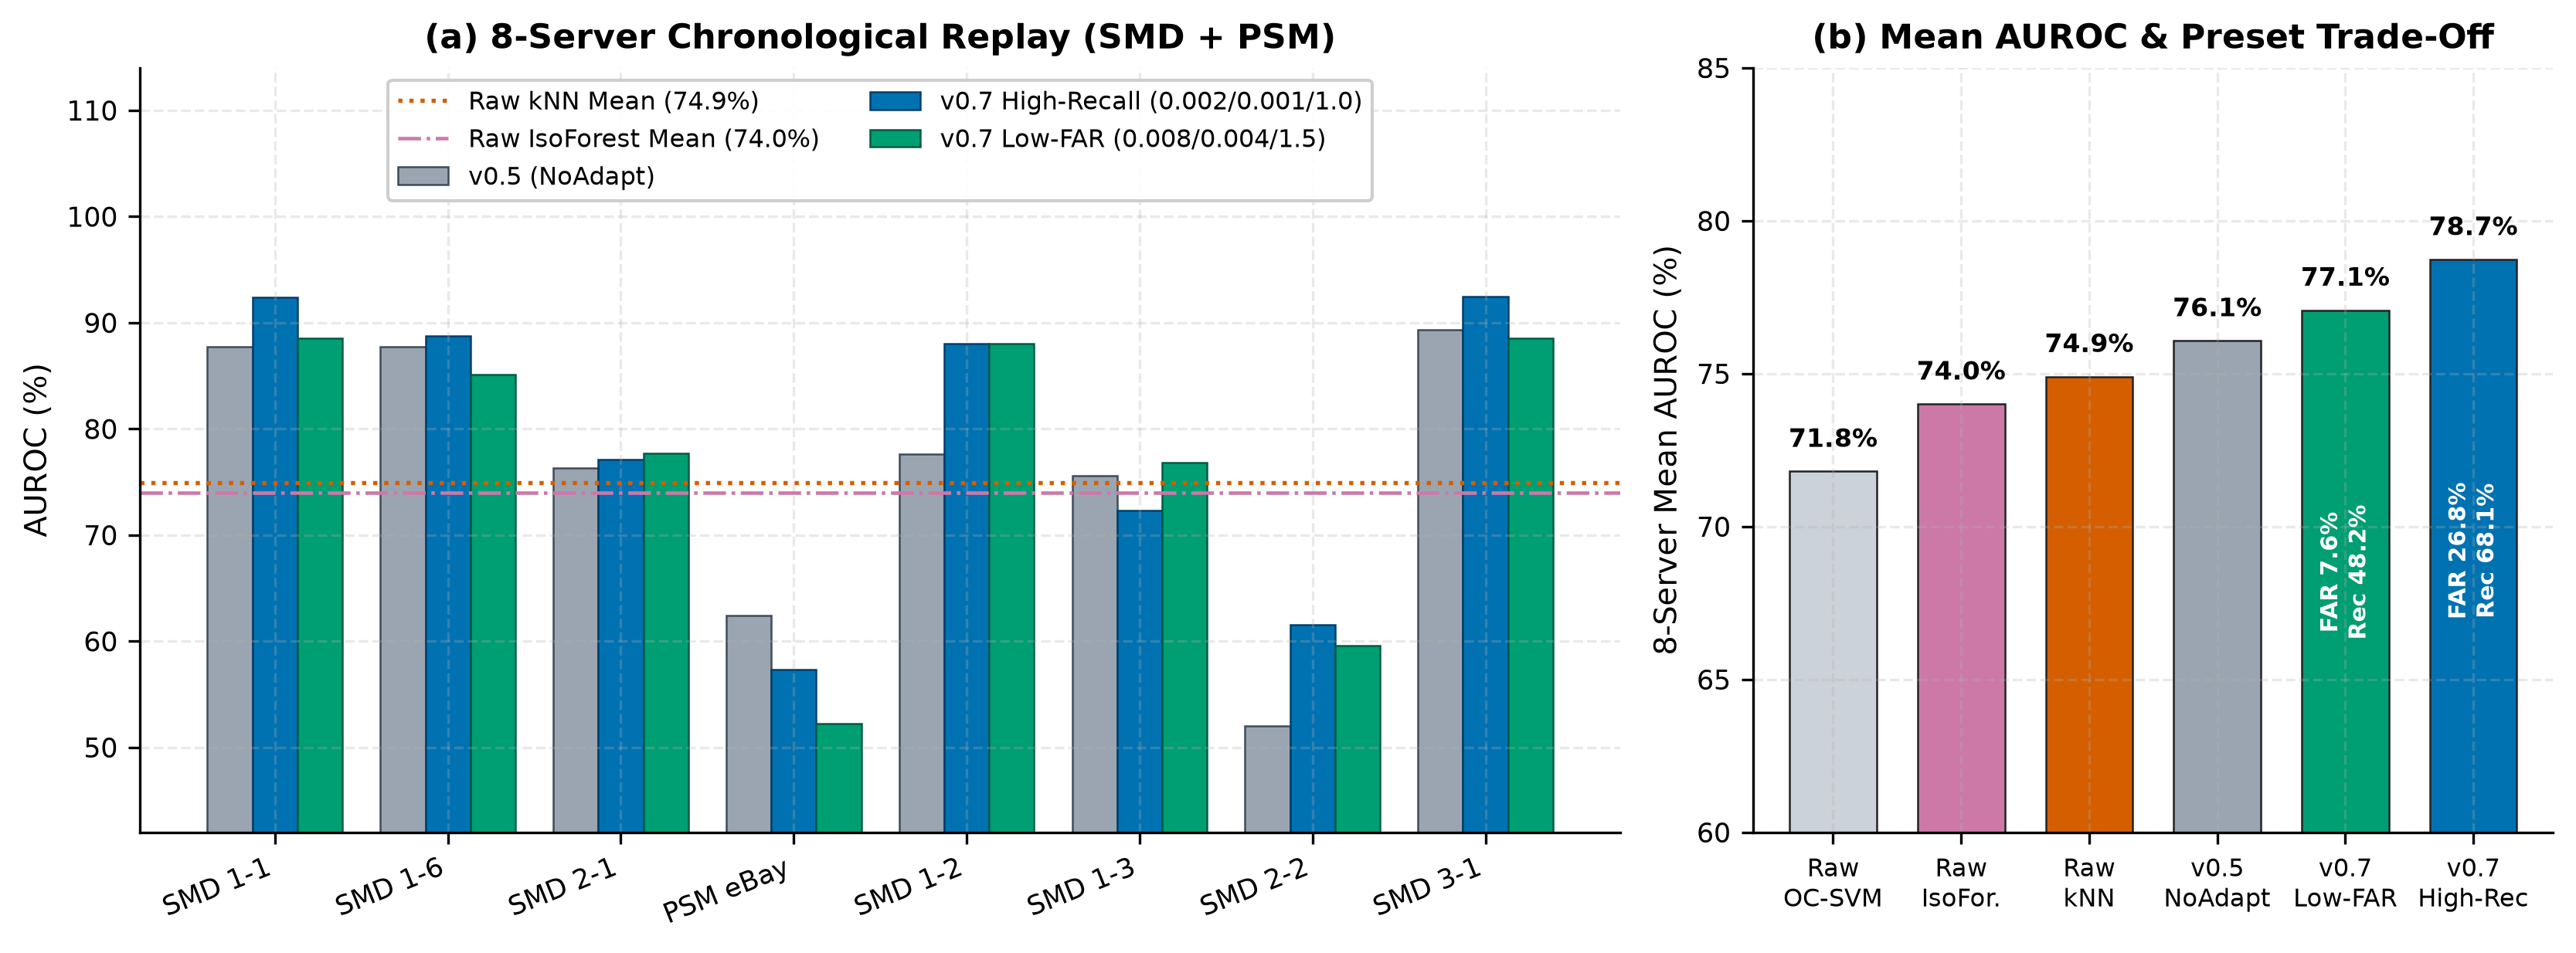
\includegraphics[width=0.96\textwidth]{fig1_8server_ablation}
  \caption{Chronological 8-server evaluation on cached SMD and PSM telemetry using locked \emph{a priori} presets. (a)~Per-server AUROC across v0.5, v0.7 High-Recall, and v0.7 Low-FAR vs.\ classical baseline means. (b)~8-server mean AUROC and explicit FAR/Recall preset trade-off.}
  \label{fig:servers}
\end{figure*}

\subsection{Cross-Device Zero-Shot vs.\ v0.7 On-Chip Auto-Warmup (Test 3B)}
Figure~\ref{fig:warmup} directly tests cross-device transfer from SMD \texttt{machine-1-1} to three unseen servers (\texttt{machine-1-2}, \texttt{machine-1-6}, \texttt{machine-2-1}). Pure zero-shot transfer scores only \textbf{29.7\%} mean AUROC because $Sim^+(d)$ invariance cannot map across heterogeneous channel topologies. Feeding just 100, 200, or 400 unlabeled normal windows directly into v0.7's on-chip \texttt{AutoCalEngineF32} state machine (zero Python threshold computation) recovers \textbf{75.3\%}, \textbf{77.8\%}, and \textbf{82.9\%} mean AUROC respectively, matching manual host calibration to 0.0 percentage points.

\begin{figure}[t]
  \centering
  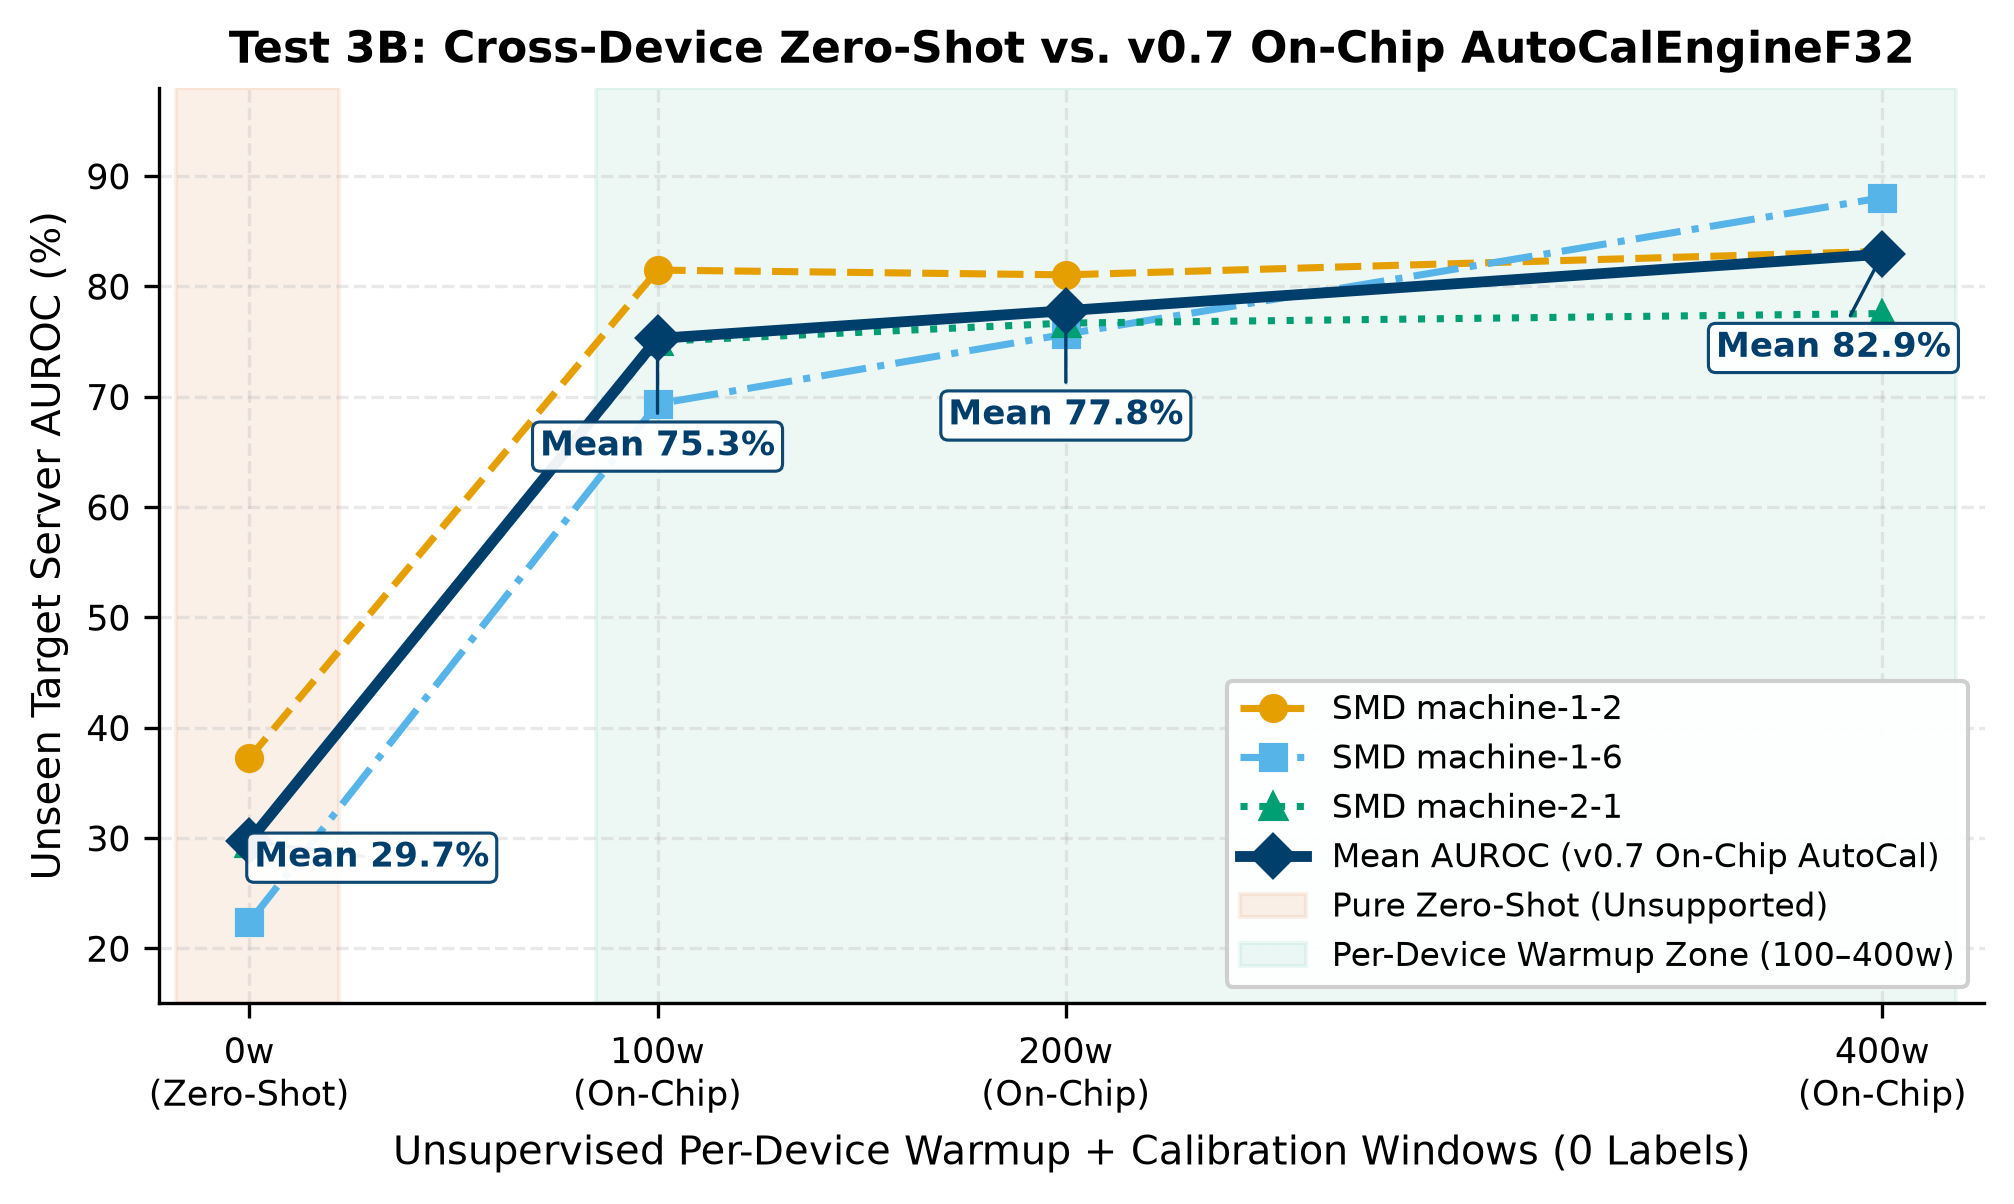
\includegraphics[width=\columnwidth]{fig2_onchip_autowarmup}
  \caption{Test 3B: Pure zero-shot transfer (29.7\%) vs.\ v0.7 on-chip \texttt{AutoCalEngineF32} zero-touch unsupervised auto-warmup (100/200/400 windows, 0 labels, 14.4\,KB static SRAM).}
  \label{fig:warmup}
\end{figure}

\subsection{Long-Duration Multi-Regime Streaming and Physical Benchmarks}
Across 50,000 windows over 5 independent held-out seeds (\texttt{[101, 202, 303, 404, 505]}) under Thermal Chip mode (Figure~\ref{fig:far}), the dual-stage alarm gate cuts false alarms by $34.8\times$ versus v0.5 (10.44\% $\to$ \textbf{0.30\% $\pm$ 0.13\%}, vs.\ 4.47\% $\pm$ 1.09\% raw 1-window) while preserving \textbf{100.0\%} fault recall (1,000/1,000 faults, 0 NaN); an abrupt $+20^\circ\text{C}$ step triggers 8/10 transition alerts and re-locks to 0.00\% steady-state FAR.

Table~\ref{tab:openml} reports verified 5-seed, 5-fold cross-conformal OpenML trajectory/physical benchmarks (\texttt{pendigits} and \texttt{PowerGrid}). Under $SO(2)$ rotation+scale, raw OC-SVM and IsoForest collapse near chance (51.1\%--56.0\%), while under mirror reflections ($\det=-1$), Gram+OC-SVM collapses to 48.5\% whereas PPC-Gauge maintains \textbf{99.2\% $\pm$ 0.6\%}.

\begin{figure*}[t]
  \centering
  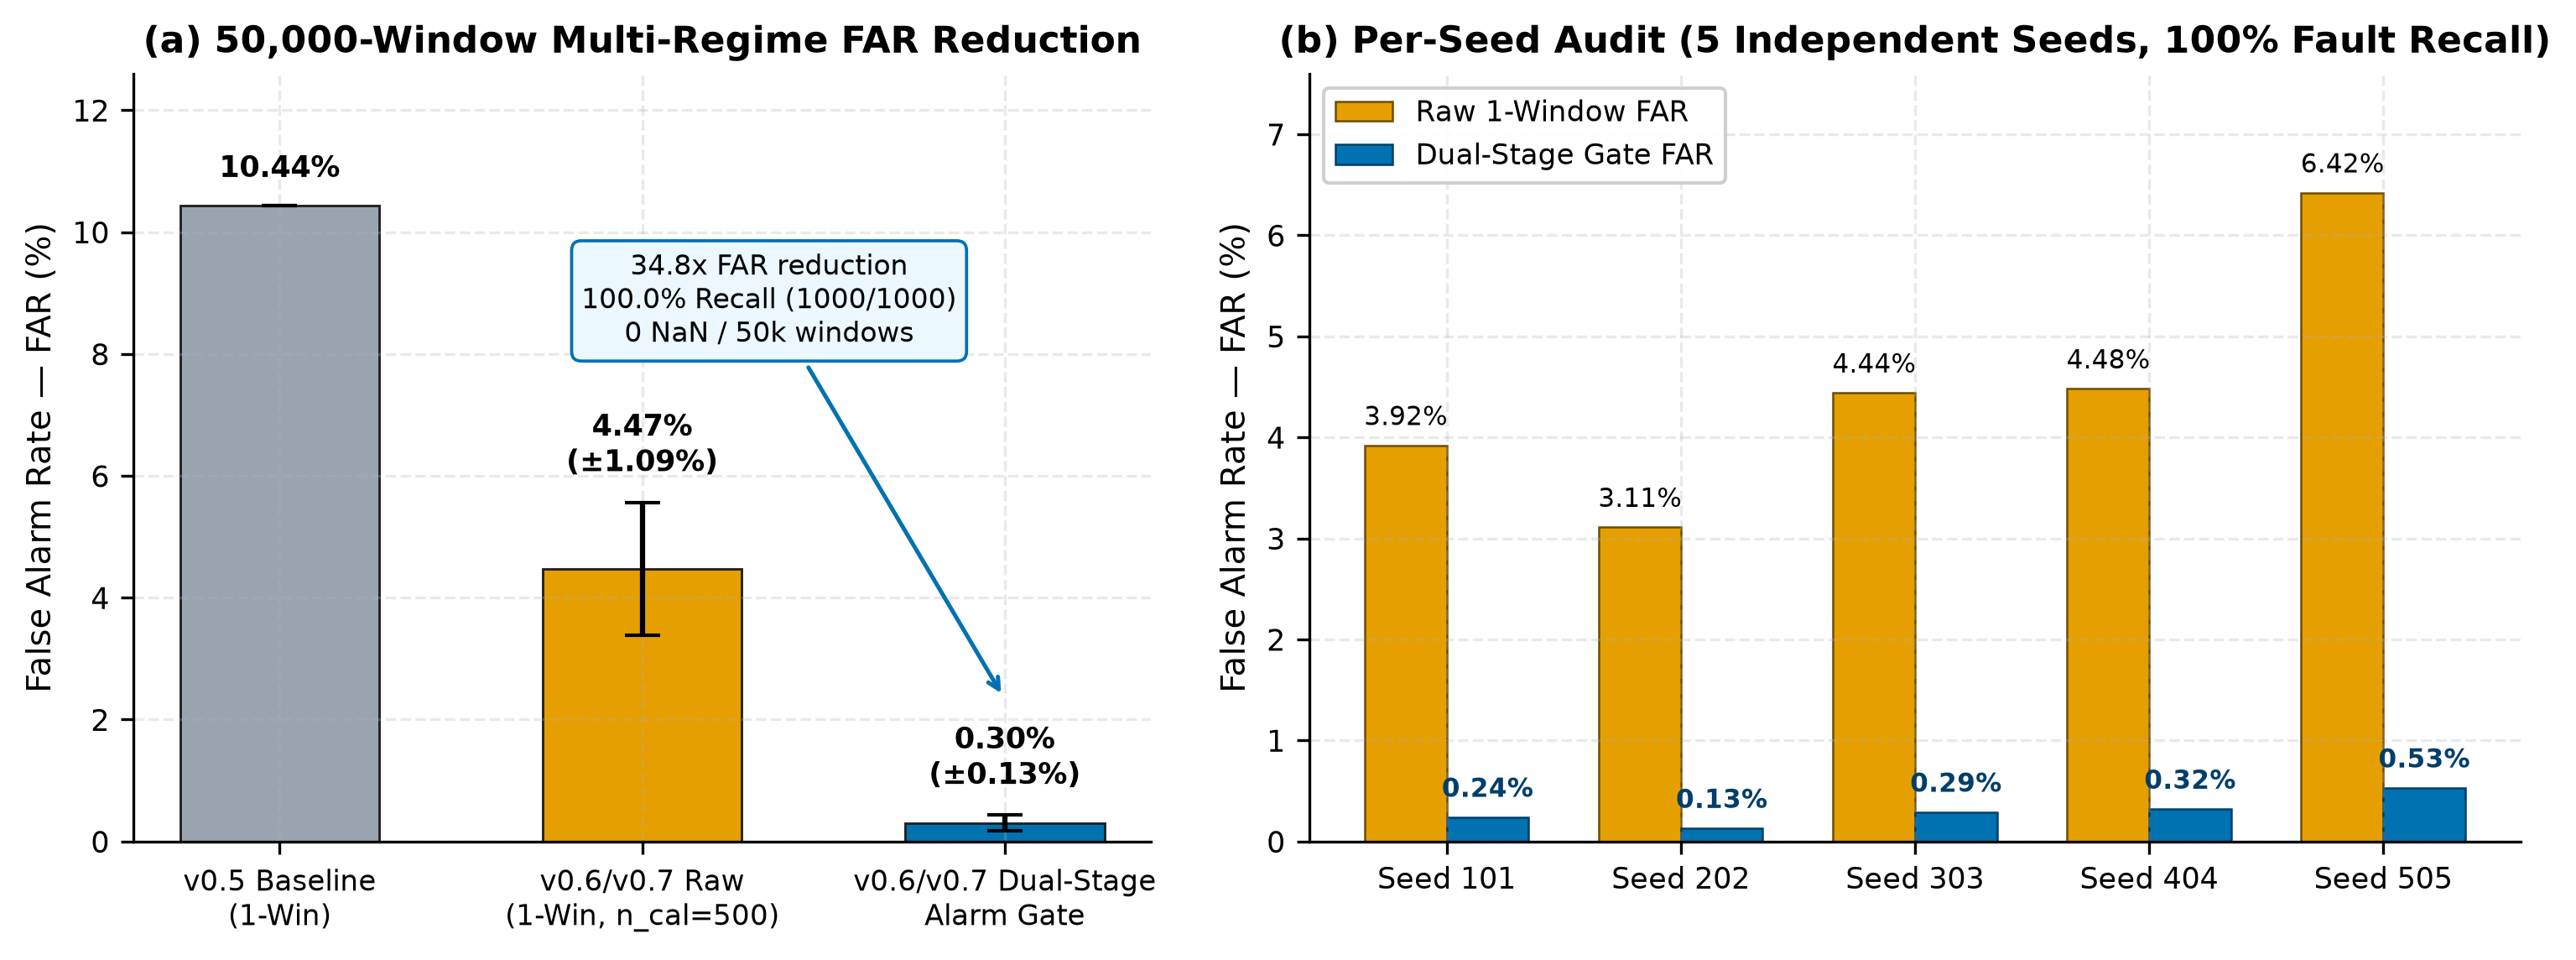
\includegraphics[width=0.92\textwidth]{fig3_dual_gate_far_reduction}
  \caption{Test 5 (50,000-window multi-regime streaming across 5 independent held-out seeds): (a)~Dual-stage alarm gate reduces FAR by $34.8\times$ vs.\ v0.5 while maintaining 100.0\% fault recall and 0 NaN; (b)~Per-seed raw 1-window vs.\ dual-stage FAR consistency.}
  \label{fig:far}
\end{figure*}

\begin{table}[t]
\centering
\caption{OpenML Physical / Trajectory Benchmarks (5 Seeds, 5-Fold AUROC \%)}
\label{tab:openml}
\begin{tabular}{@{}lcccc@{}}
\toprule
\textbf{Scenario} & \textbf{OC-SVM} & \textbf{IsoFor.} & \textbf{Gram+SVM} & \textbf{PPC-Gauge} \\
\midrule
\texttt{pendigits} Upright & 96.7$\pm$1.3 & 96.5$\pm$1.0 & 94.6$\pm$1.0 & \textbf{98.8$\pm$0.8} \\
\texttt{pendigits} $SO(2)$+Scale & 51.1$\pm$3.5 & 56.0$\pm$4.4 & 94.6$\pm$1.0 & \textbf{98.8$\pm$0.8} \\
\texttt{pendigits} Mirror ($\det\!=\!-1$) & 53.3$\pm$2.3 & 49.2$\pm$3.6 & 48.5$\pm$2.1 & \textbf{99.2$\pm$0.6} \\
\texttt{PowerGrid} $8\!\times\!4$ Load+$SO(4)$ & 50.0$\pm$0.0 & 52.3$\pm$2.9 & 65.3$\pm$3.9 & \textbf{75.5$\pm$3.4} \\
\texttt{PowerGrid} $8\!\times\!2$ Load+$SO(2)$ & 50.3$\pm$0.2 & 49.8$\pm$3.1 & 68.0$\pm$3.4 & \textbf{78.8$\pm$3.9} \\
\bottomrule
\end{tabular}
\end{table}

\subsection{Cross-Compilation and Host CPU Software Throughput}
Continuous integration verifies 5/5 cross-compilation targets: Linux x86-64 (\texttt{std} \texttt{cdylib} and \texttt{\#![no\_std]}), ARM Cortex-M4F (\texttt{thumbv7em-none-eabihf}, \texttt{\#![no\_std]}), Linux ARM64 (\texttt{aarch64-unknown-linux-gnu}), and Windows x86-64 GNU (\texttt{x86\_64-pc-windows-gnu}), plus C99 ABI compilation and execution of \texttt{examples/c\_stream\_demo.c}. Criterion micro-benchmarks on an AMD64 Windows host (\texttt{benches/triad\_bench.rs}; \emph{host software CPU timing only, not MCU silicon}) measure: \texttt{canonicalize\_8x4} = \textbf{567\,ns}, \texttt{step\_v61} score-only = \textbf{973\,ns}, live learn+score = \textbf{1.84\,$\mu$s}, \texttt{AutoCalEngineF32} Monitor step = \textbf{1.13\,$\mu$s}, and full 400-window on-chip warmup+calibration = \textbf{749\,$\mu$s}.

\section{Design Boundaries, Limitations, and Level 3 Hardware Protocol}
To maintain strict scientific integrity, we state four explicit design boundaries:
\begin{enumerate}
  \item \textbf{Per-Device Unsupervised Warmup Requirement:} Pure zero-shot transfer across heterogeneous devices is unsupported (29.7\% AUROC). Deployment requires 100--400 normal unlabeled warmup windows per device.
  \item \textbf{Domain of Advantage:} PPC-Gauge-Triad targets ultra-constrained \texttt{\#![no\_std]} MCU/edge streaming ($<16$\,KB SRAM, 0\,B heap, $Sim^+(d)$ and chiral robustness). We do not claim superiority over heavy deep or offline models on unconstrained cloud hardware.
  \item \textbf{Non-Stationary Server Drift Trade-Off:} Under severe train-to-test DC shifts (e.g., SMD \texttt{machine-1-6}, PSM), operators must choose between High-Recall and Low-FAR presets \emph{a priori}; raw single-window scores without persistence gating should not trigger automated shutdowns.
  \item \textbf{Level 3 Physical Silicon Verification (\textbf{PENDING}):} No physical MCU/FPGA cycle count, \texttt{.map} Flash footprint, or mW power consumption is claimed in this preprint. External hardware teams can execute physical silicon benchmarks directly using our open ARMv7E-M CoreSight DWT evaluation template (\texttt{examples/level3\_cortex\_m4f\_eval\_template.rs}) together with \texttt{probe-rs}/\texttt{defmt}, \texttt{arm-none-eabi-size}, and an inline power profiler.
\end{enumerate}

\section{Conclusion and Reproducibility}
PPC-Gauge-Triad v0.7 demonstrates that exact $Sim^+(d)$ canonicalization, chirality-sensitive anomaly scoring, zero-inversion precision tracking, and complete zero-touch on-chip split-conformal auto-warmup fit within \textbf{14.40\,KB} of static SRAM in \texttt{\#![no\_std]} Rust with zero heap allocation. All Rust Level~1 tests, Criterion benchmarks, C99 ABI headers, cached offline SMD/PSM scripts, figure generators, and the Cortex-M4F Level~3 evaluation template are reproducibly packaged in the project repository.

\begin{thebibliography}{5}
\bibitem{su2019omni}
Y.~Su \emph{et al.}, ``Robust anomaly detection for multivariate time series through stochastic recurrent neural network,'' in \emph{Proc. ACM SIGKDD}, 2019, pp. 2828--2837.

\bibitem{abdulaal2021psm}
A.~Abdulaal, Z.~Liu, and T.~Lancewicki, ``Practical approach to asynchronous multivariate time series anomaly detection and localization,'' in \emph{Proc. ACM SIGKDD}, 2021, pp. 2485--2494.

\bibitem{vovk2005conformal}
V.~Vovk, A.~Gammerman, and G.~Shafer, \emph{Algorithmic Learning in a Random World}. Springer, 2005.

\bibitem{golub2013matrix}
G.~H. Golub and C.~F. Van~Loan, \emph{Matrix Computations}, 4th~ed. Johns Hopkins Univ.\ Press, 2013.

\bibitem{sherman1950}
J.~Sherman and W.~J. Morrison, ``Adjustment of an inverse matrix corresponding to a change in one element of a given matrix,'' \emph{Ann.\ Math.\ Stat.}, vol.~21, no.~1, pp. 124--127, 1950.
\end{thebibliography}

\end{document}
